\section{Simulación}

El modelo matemático obtenido se implementó en MATLAB 
para estudiar el comportamiento del sistema.
La tabla \ref{table: simulation conditions}
muestra las condiciones de simulación del programa.
El código del programa se encuentra disponible en 
GitHub\footnote{\url{https://github.com/der-coder/Cinvestav-SystemModeling-project/tree/master/codigosM}}
y se incluye como anexo.

\begin{table}[hb]
 \begin{center}
\begin{tabular}{lc}
\hline
Longitud ($l$) & 0.3 [m] \\
Masa ($m$) & 0.12166 [kg]\\
Coeficiente de fricción ($k$) & $\{0,0.1\}$ [$N \cdot s / m$] \\
Posición angular inicial ($\theta_0$) & $0.5\pi$ [rad] \\
Velocidad angular inicial ($\dot{\theta}$) & 0 [rad/s] \\
Tiempo de simulación & 10 [s]  \\
Gravedad ($g$) & 9.81 [$m/s^2$]  \\
\hline
 \end{tabular}
 \end{center}
 \caption{Condiciones de simulación del sistema.}
\label{table: simulation conditions}
\end{table}

\subsection{Caso sin fricción}

Para el caso sin fricción, el péndulo describe 
el comportamiento armónico simple. 
Observamos que la posición angular y la velocidad angular
varían periódicamente (figura \ref{fig: time plot theta dtheta no friction}), y la amplitud máxima
del período es el mismo para cada uno de ellos.

La ausencia de fricción en el sistema no permite al sistema
encontrar un estado de reposo o estabilización. 
Esto se observa en la figura \ref{fig: phase plot theta no friction}, que
muestra el diagrama de fase del sistema.
El comportamiento del sistema describe una elipse para todos los períodos del sistema.


\begin{figure}[hb!]
 \centering 
 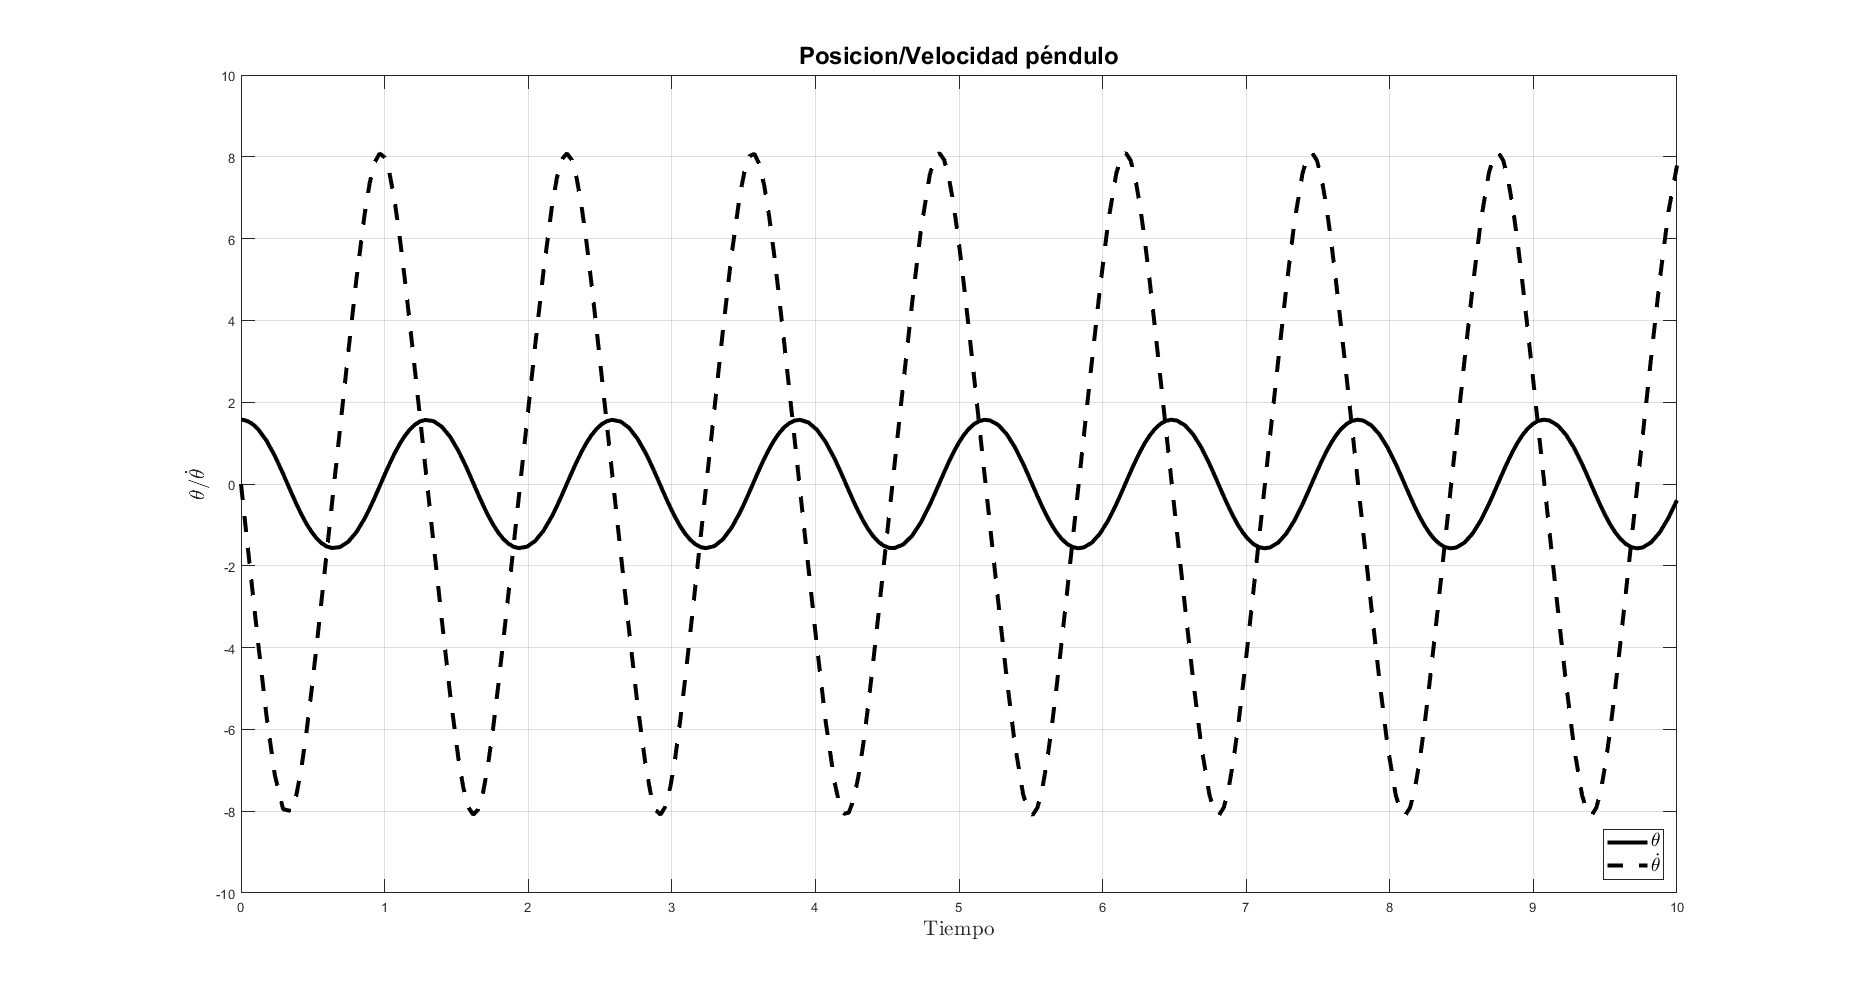
\includegraphics[scale=0.2]{./img/PosVelNF.png}
 % fasependulox2.png: 1853x1003 px, 96dpi, 49.02x26.53 cm, bb=0 0 1390 752
 \caption{Comportamiento de $\theta(t)$ y $\dot{\theta}(t)$ en el tiempo sin fricción.}
 \label{fig: time plot theta dtheta no friction}
\end{figure}

\begin{figure}[hb!]
 \centering 
 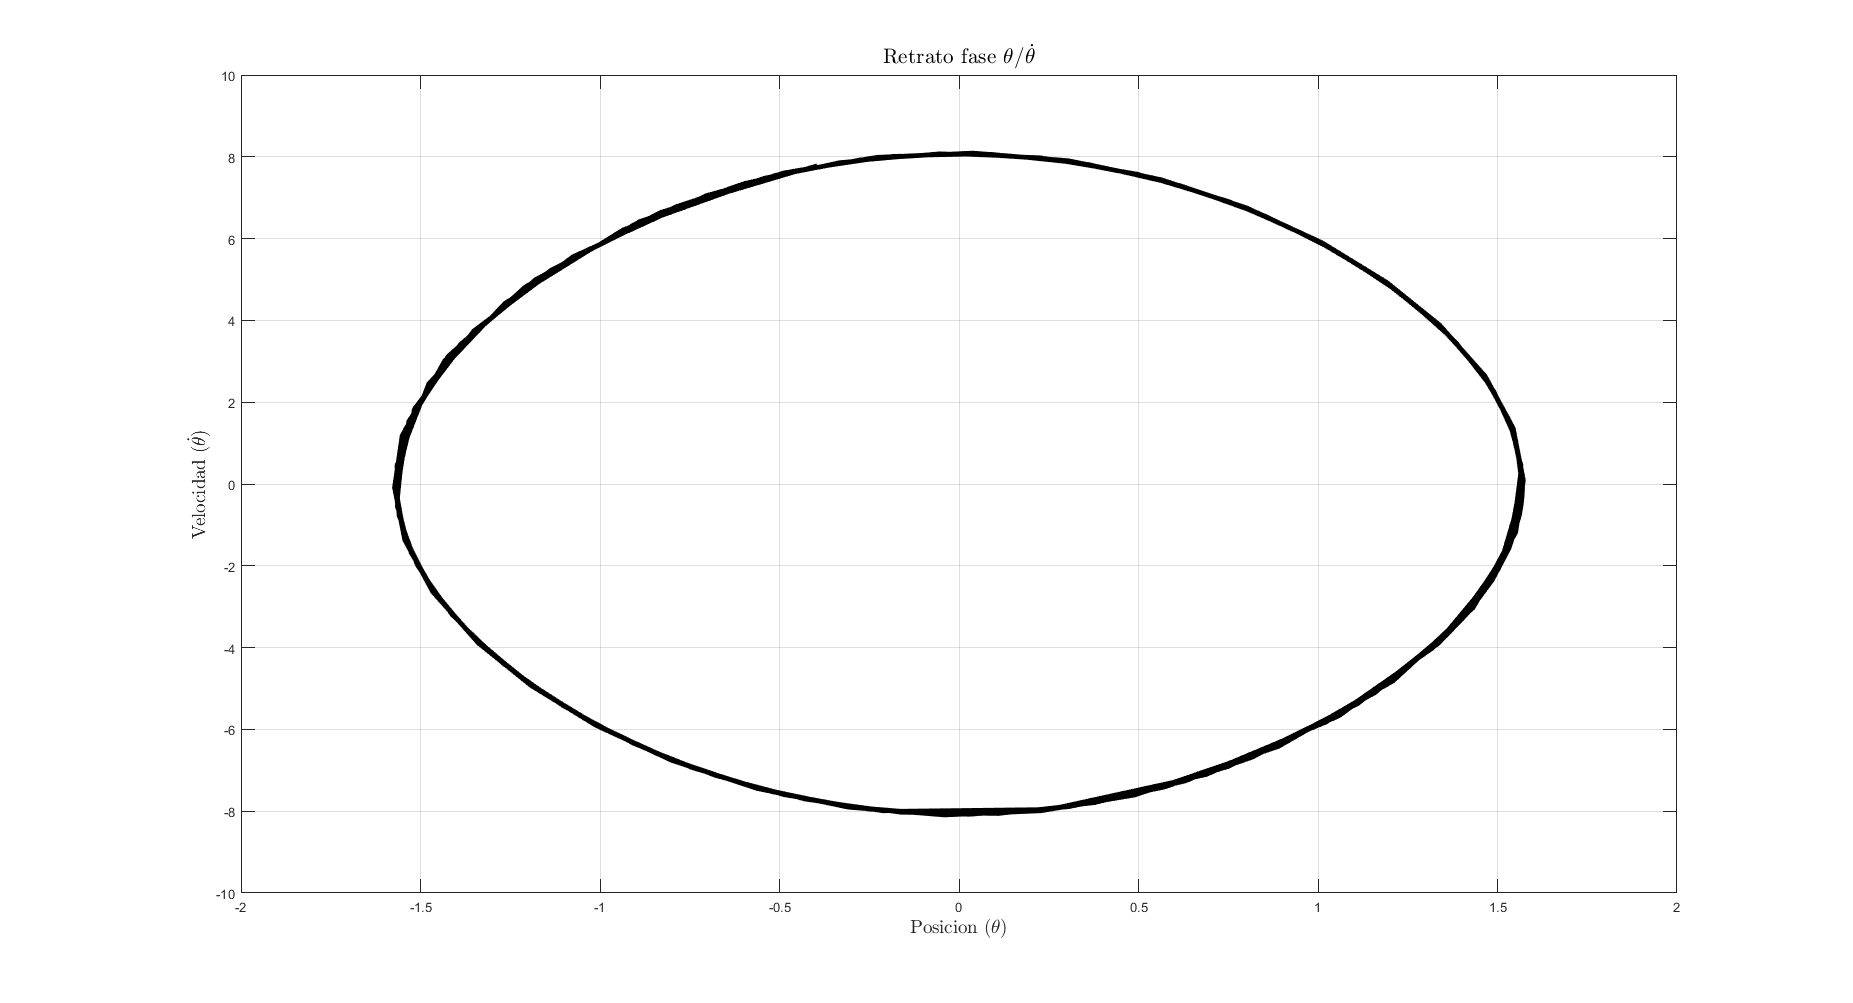
\includegraphics[scale=0.2]{./img/faseNF.png}
 % fasependulox2.png: 1853x1003 px, 96dpi, 49.02x26.53 cm, bb=0 0 1390 752
\caption{Diagrama de fase de $\theta(t)$ y $\dot{\theta}(t)$ sin fricción.}
 \label{fig: phase plot theta no friction}
\end{figure}

\pagebreak

\subsection{Caso con fricción}

Se observa que el péndulo tiende a una posición de reposo debido
al efecto que la fuerza de fricción tiene sobre el sistema.
El péndulo comienza en la posición angular máxima posible 
($\theta_{max}$) y la amplitud de las crestas y valles de las 
ecuaciones disminuye para cada período de oscilación. 
Esto puede ser observado en la figura \ref{fig: time plot theta dtheta friction}.
Se observa que conforme \emph{t} se aproxima a infinito, 
la posición angular del sistema tiende al valor cero.


El diagrama de fase, mostrado en la figura 
\ref{fig: phase plot theta friction}, confirma esta tendencia.
La curva del sistema indica que tiende 
a un punto de estabilización en $\theta = 0$,
posicionando al péndulo en el eje vertical 
del marco referencial.

\begin{figure}[hb!]
 \centering 
 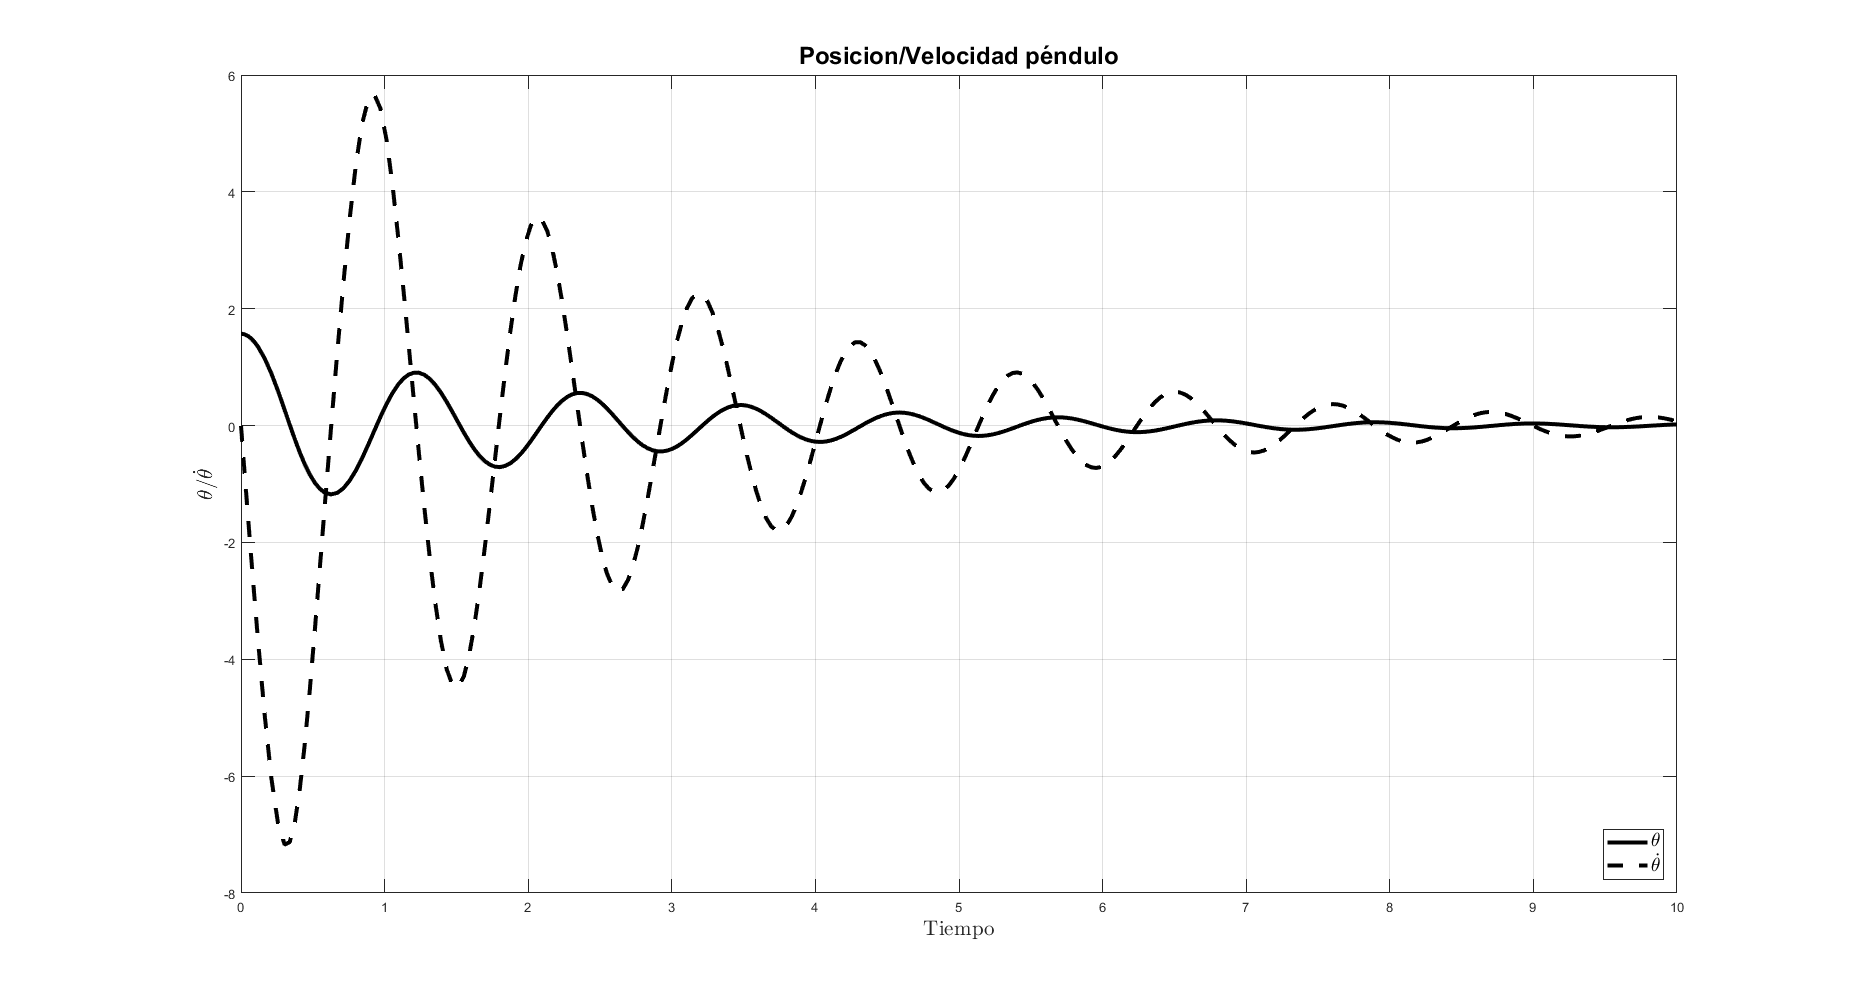
\includegraphics[scale=0.3]{./img/PosVelF.png}
 % fasependulox2.png: 1853x1003 px, 96dpi, 49.02x26.53 cm, bb=0 0 1390 752
 \caption{Comportamiento de $\theta(t)$ y $\dot{\theta}(t)$ en el tiempo.}
 \label{fig: time plot theta dtheta friction}
\end{figure}

\begin{figure}[hb!]
 \centering 
 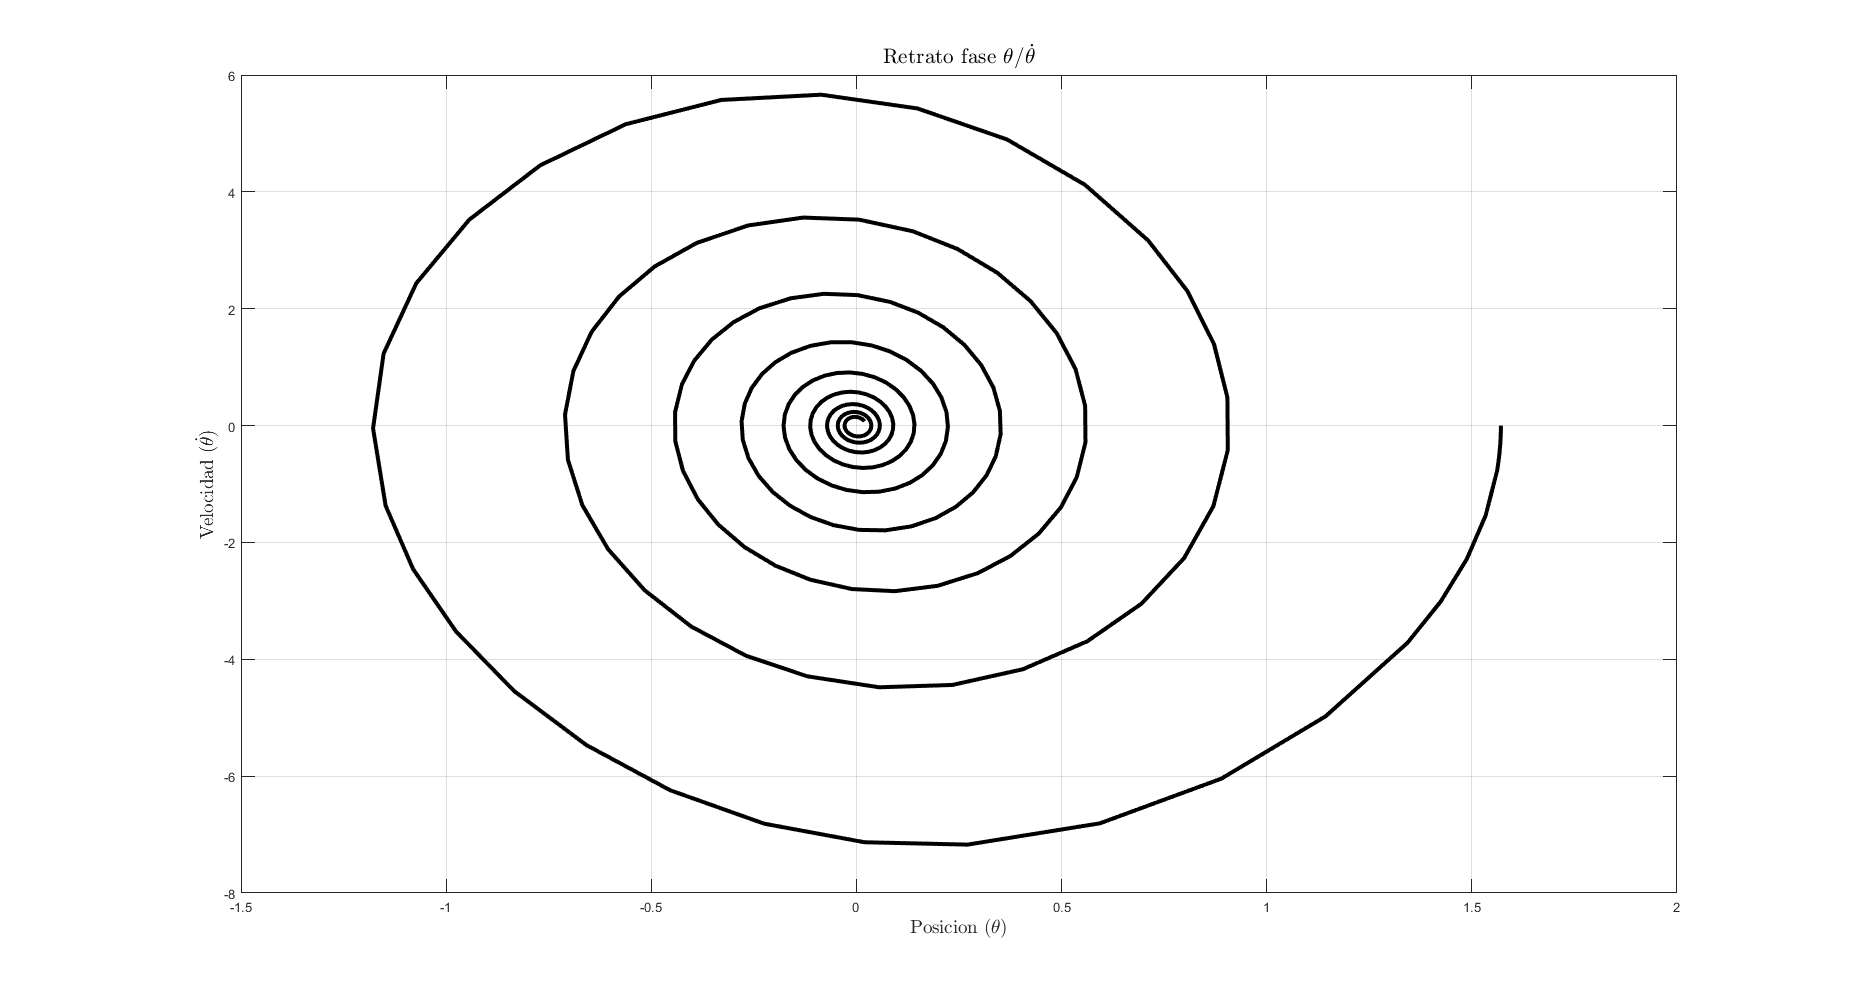
\includegraphics[scale=0.3]{./img/faseF.png}
 % fasependulox2.png: 1853x1003 px, 96dpi, 49.02x26.53 cm, bb=0 0 1390 752
\caption{Diagrama de fase de $\theta(t)$ y $\dot{\theta}(t)$.}
 \label{fig: phase plot theta friction}
\end{figure}
